\documentclass[10pt, letterpaper]{article}

% %%%%%%%%% Packages %%%%%%%%%%
\usepackage[empty]{fullpage}
\usepackage{geometry}
\usepackage{fontawesome5}
\usepackage{ragged2e}
\usepackage{graphicx}
\usepackage{xcolor}
\usepackage{titlesec}
\usepackage[hidelinks]{hyperref}
\usepackage{tabularx}
\usepackage{enumitem}
\usepackage{multicol}
\usepackage[spanish]{babel}

% Settings
\geometry{lmargin=1cm,rmargin=1cm,tmargin=0.5cm,bmargin=0.5cm}
\urlstyle{same}

%% Section formatting
\titleformat{\section}{\centering\large}{}{0cm}{}[\titlerule]

%% News Commands
\newcommand{\CVName}[1]{\textbf{\Large #1} \\[3mm]}
\newcommand{\CVLocation}[1]{{\footnotesize \faMapMarked*} #1 \\}
\newcommand{\CVMobile}[1]{{\footnotesize \faMobile*} #1 \\}
\newcommand{\CVEmail}[1]{{\footnotesize \faEnvelope[regular] } \href{mailto:#1}{#1} \\}
\newcommand{\CVLinkedin}[1]{{\footnotesize \faLinkedin}\ \url{#1} \\}
\newcommand{\CVGithub}[1]{{\footnotesize \faGithub}\ \url{#1} \\}

\newcommand{\CVitem}[1]{
	\item \small{#1}
}
\newcommand{\CVListStart}{\begin{itemize}[leftmargin=0cm, label={}]}
\newcommand{\CVListEnd}{\end{itemize}}
\newcommand{\CVSubHeading}[4]{
	\item \begin{tabular*}{19.5cm}[t]{l@{\extracolsep{\fill}}r}
		\textbf{#1} & #2 \\
		\small #3 & \small #4 \\
	\end{tabular*} \vspace{-4pt}
}
\newcommand{\CVItemizeStart}{\begin{itemize}[rightmargin=1cm, label={\tiny \textbullet}]}
\newcommand{\CVItemizeEnd}{\end{itemize}}


\begin{document}
\begin{minipage}[c]{2.5cm}
	\vspace{6mm}
	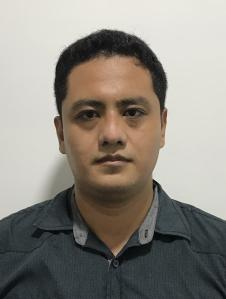
\includegraphics[width=2.5cm, height=3.3cm]{../images/fotocv.jpg}
	\hfill
	\vrule
	\hfill
\end{minipage}
\begin{minipage}[c]{15cm}
	\center
	\CVName{Edwin Enrique Pérez Rodríguez}
	\CVLocation{Mérida, México}
	%\CVMobile{9932885771}
	\CVEmail{edwin.epr.219@gmail.com}
	\CVLinkedin{https://www.linkedin.com/in/edwin-epr/}
	\CVGithub{https://github.com/EdHeny}
\end{minipage}

\section*{Perfil Profesional}
Matemático con Maestría en Ciencia e Ingeniería de la Computación, orientado a Data Engineering, con experiencia práctica diseñando pipelines ETL, automatizando flujos de datos y gestionando infraestructura en entornos de cómputo científico de alto rendimiento. Combino una sólida base analítica con habilidades en Python, Java, SQL, Google Cloud Platform y CI/CD para construir soluciones de datos robustas y escalables. Busco aplicar este perfil en equipos de tecnología donde los datos sean un activo estratégico.
\section{Educación}
\CVListStart
\CVSubHeading{Universidad Nacional Autónoma de México}{CDMX, México}{Maestría en Ciencia e Ingeniería de la Computación (Titulado)}{Agosto 2021 - Julio 2023}
\CVSubHeading{Universidad Juárez Autónoma de Tabasco}{Villahermosa, México}{Licenciatura en Matemáticas (Titulado)}{Agosto 2016 - Junio 2020}
\CVListEnd
% \section{Proyectos}
% \CVListStart
% %
% \CVSubHeading{IXCHEL2D}{}{Software de simulación computacional para problemas de termofluidos}{}
% \CVItemizeStart
% \CVItemizeEnd
% %
% \CVSubHeading{ParCFD 2025 Conference Website}{ }{Sitio web completo para la 36th Parallel CFD international conference 2025}{ }
% \CVItemizeStart
% \CVItemizeEnd
% %
% \CVSubHeading{Sitio web DeMAG}{ }{Sitio web institucional del Departamento de Matemáticas Aplicadas y Geociencias, UNAM}{ }
% \CVItemizeStart
% \CVItemizeEnd
% %
% \CVSubHeading{GitHub DeMAG}{ }{Repositorio de código del Departamento de Matemáticas Aplicadas y Geociencias, UNAM}{ }
% \CVItemizeStart
% \CVItemizeEnd
%
% \CVListEnd
\section{Experiencia Profesional}
\CVListStart
\CVSubHeading{\small Técnico Académico Asociado C}{Febrero 2024 - a la fecha}{ENES Mérida UNAM}{Mérida, México}
\CVItemizeStart
\CVitem{Construí pipelines ETL automatizados en Python y MATLAB para ingestar y procesar más de 32 GB de datos oceanográficos y meteorológicos desde servidores externos, eliminando descargas manuales para el equipo de investigación.}
\CVitem{Automaticé el build system de Ixchel 2D con CMake, ahorrando ~30 minutos diarios de configuración manual y reduciendo errores de entorno al estandarizar la alternancia entre arquitecturas GPU (OpenACC) y Multicore.}
\CVitem{Desarrollé y mantuve la plataforma web de la 36th Parallel CFD International Conference (\href{https://www.parcfd2025.org/}{parcfd2025.org}) con CI/CD en GitHub Actions, dando soporte a 45 asistentes internacionales e integrando ConfTool para gestión de abstracts y registros.}
\CVitem{Diseño y mantengo el sitio web institucional del DeMAG (\href{https://www.demag.enesmerida.unam.mx/}{demag.enesmerida.unam.mx}) con Jekyll y GitHub Actions, sirviendo como canal oficial para 10 investigadores y 20 estudiantes.}
\CVitem{Centralicé 10 repositorios de software científico en la primera GitHub Organization del DeMAG, habilitando la colaboración de 10 investigadores y la distribución de recursos a 20 estudiantes.}
\CVitem{Diseñé e impartí talleres de programación integrados al currículo de Introducción a la Geodinámica y Análisis de Datos Geofísicos, capacitando a 12 estudiantes en herramientas computacionales para análisis científico.}
\CVItemizeEnd

\CVSubHeading{\small Profesor de Matemáticas}{Agosto 2022 - Diciembre 2022}{NUMERALIA}{Villahermosa, México}
\CVItemizeStart
\CVitem{Impartí asesorías personalizadas de matemáticas y física a 23 estudiantes de niveles básico, preparatoria y universitario, logrando la nivelación de competencias clave según los objetivos curriculares de cada nivel.}
\CVItemizeEnd

\CVSubHeading{\small Ayudante de Profesor}{ Enero 2023 - Junio 2023}{Facultad de Ciencias UNAM}{CDMX, México}
\CVItemizeStart
\CVitem{Diseñé e impartí un taller de Estructuras Avanzadas de Datos en Python para 8 estudiantes de Actuaría, apoyando la comprensión de algoritmos aplicados a Investigación de Operaciones.}
\CVItemizeEnd

\CVListEnd

\newpage
\section{Cursos y Formación Complementaria}
\CVListStart
\CVSubHeading{Java Developer Professional}{Completado: Junio 2025}{CodeGym University}{En línea}
\CVItemizeStart
\CVitem{Curso intensivo de 12 meses, 8 proyectos, más de 1,000 ejercicios, Spring Boot, Hibernate, Docker, REST API, SQL, JUnit, Mockito.}
\CVItemizeEnd
\CVListEnd
\section{Habilidades}
\CVListStart
%
\CVSubHeading{Lenguajes de Programación:}{}{}{}
\vspace{-15pt}
\CVItemizeStart
\begin{multicols}{5}
	\CVitem{Python}
	\CVitem{Java}
	\CVitem{MATLAB}
	\CVitem{Bash}
	\CVitem{SQL}
	\CVitem{C}
	\CVitem{Fortran}
\end{multicols}
\CVItemizeEnd
%
\CVSubHeading{Ingeniería de Datos y DevOps:}{}{}{}
\vspace{-15pt}
\CVItemizeStart
\begin{multicols}{3}
	\CVitem{Pipelines de Datos (ETL)}
	\CVitem{Integración de APIs}
	\CVitem{PostgreSQL}
	\CVitem{Docker}
	\CVitem{Git}
	\CVitem{GitHub Actions (CI/CD)}
	\CVitem{GitHub Organization Management}
\end{multicols}
\CVItemizeEnd
%
\CVSubHeading{Cloud}{}{}{}
\vspace{-12pt}
\CVItemizeStart
\CVitem{Google Cloud Platform (BigQuery, Cloud Storage, Cloud Functions, Compute Engine)}
\CVItemizeEnd
%
\CVSubHeading{Desarrollo Web}{}{}{}
\vspace{-15pt}
\CVItemizeStart
\begin{multicols}{3}
	\CVitem{Spring Framework}
	\CVitem{Spring Boot}
	\CVitem{Hibernate}
	\CVitem{Jekyll}
	\CVitem{Bulma CSS}
\end{multicols}
\CVItemizeEnd
%
\CVSubHeading{Cómputo científico y GPU}{}{}{}
\vspace{-15pt}
\CVItemizeStart
\begin{multicols}{4}
	\CVitem{CUDA}
	\CVitem{OpenACC}
	\CVitem{OpenMP}
	\CVitem{CMAKE (Build Systems)}
\end{multicols}
\CVItemizeEnd
%
\CVSubHeading{Testing}{}{}{}
\vspace{-15pt}
\CVItemizeStart
\begin{multicols}{2}
	\CVitem{JUnit}
	\CVitem{Mockito}
\end{multicols}
\CVItemizeEnd
%
\CVSubHeading{Idiomas}{}{}{}
\vspace{-12pt}
\CVItemizeStart
\CVitem{Español (Nativo)}
\CVitem{Inglés (Lectura técnica avanzada. escritura y conversación intermedia.)}
\CVItemizeEnd
%
\CVSubHeading{Liderazgo y Educación:}{}{}{}
\vspace{-15pt}
\CVItemizeStart
\begin{multicols}{3}
	\CVitem{Capacitación Técnica \\ (Technical Training)}
	\CVitem{Diseño de talleres}
	\CVitem{Mentoría académica}
	\CVitem{Colaboración transfuncional}
\end{multicols}
\CVItemizeEnd
%
\CVListEnd
%\section{Actividades Académicas}
%\CVItemizeStart
%\CVitem{Tomé el curso virtual <<Fundamentos de la modelación matemática: Un acercamiento a la  epidemiología matemática>> impartido por la Sociedad Mexicana de Computación Científica y  sus Aplicaciones, los días 25, 30 de junio y 2 de julio del 2020, con una duración de 5 horas.}
%\CVitem{Presenté la ponencia <<Resolución Numérica de la Ecuación de Poisson en 2D>> en XII Foro de
%	Matemáticas del Sureste llevado a cabo del 9 al 13 de septiembre de 2019 en Cunduacán,
%	Tabasco.}
%\CVitem{Tomé el curso «El método de elemento finito para la solución de la ecuación de calor» en el
%	marco del XII Foro de Matemáticas del Sureste, con una duración de 4 horas.}
%\CVitem{Presenté la ponencia «Resolución Numérica de la Ecuación de Poisson en 2D» en XXVIII
%	Escuela Nacional de Optimización y Análisis Numérico llevado a cabo del 26 al 30 de agosto
%	de 2019 en Zacatecas, Zacatecas.}
%\CVitem{Participé en el equipo organizador del 51 Congreso Nacional de la Sociedad Mexicana de
%	Matemáticas llevado a cabo del 21 al 26 de octubre de 2018 en Villahermosa, Tabasco.}
%\CVitem{Participé con el cartel “Tratamiento óptimo del VIH al maximizar la respuesta inmune”, en el
%	Congreso Sur-sureste de Matemáticas 2017 llevado a cabo del 20 al 24 de noviembre en
%	Oaxaca, Oaxaca.}
%\CVItemizeEnd
\end{document}
